\begin{exercice}[Par paires]
Regroupe par deux les expressions qui sont égales.
\begin{colenumerate}{2}
\item $A = 6x^2 + 4$
\item $B = 6x^2 + 2$
\item $C = 3x^2(2x + 4)$
\item $D = 3(2x^2 + 1) - 1$
\item $E = 6x(x^2 + 2x)$
\item $F = 8x^2 - 4 - 2x^2 + 8$
\end{colenumerate}
\end{exercice}

\begin{exercice}[Une expression en trop]
Trouve l'intrus.
\begin{colenumerate}{2}
\item $A = 4(2x - 3)$
\item $B = 8x - 12$
\item $C = 5(x - 4) + 3x + 8$
\item $D = 10(x - 1) - 2x$
\item $E = 6(2x - 3) + 2(3 - 2x)$
\end{colenumerate}
\end{exercice}

\begin{exercice}[Substitution]
Soit $G = 3(4x - 2)$. Calcule $G$ lorsque :

\begin{colenumerate}{2} 
\item $x = 5$
\item $4x - 2 = 7$
\item $12x = 11$
\item $6x = 5$
\item $2x - 1 = 3$
\item $3x = 25$
\end{colenumerate} 
\end{exercice}

\begin{exercice}[]
\textsl{Marie dit qu'en ajoutant deux nombres impairs, on obtient toujours un nombre impair.}

\begin{colenumerate}{1} 
\item Prouve-lui qu'elle a tort à l'aide d'un contre-exemple.
\item \ref{DisEA01} En utilisant la variable $n$, écris une expression désignant un nombre pair puis une autre désignant un nombre impair.
\item Utilise la question \label{DisEA01} pour démontrer à Marie que la somme de deux nombres impairs n'est jamais impaire.
\end{colenumerate} 
\end{exercice}

\begin{exercice}[Au zoo]
Au zoo, il y a des cacatoès et des koalas. On peut y dénombrer 50 têtes et 140 pattes.

\begin{colenumerate}{1} 
\item Si besoin, recherche, dans un dictionnaire ou sur internet, le nombre de pattes d'un cacatoès et d'un koala.
\item On note $c$ le nombre de cacatoès. Exprime le nombre de koalas en fonction de $c$.
\item Écris une expression $P$ représentant le nombre de pattes en fonction de $c$.
\item Développe puis réduis $P$.
\item Calcule le nombre de cacatoès puis le nombre de koalas.
\end{colenumerate} 
\end{exercice}

\begin{exercice}[Un carré qui grandit]
Soit ABCD un carré de 5\,cm de côté. 

\begin{colenumerate}{1} 
\item Calcule le périmètre $\mathcal{P}_1$ et l'aire $\mathcal{A}_1$ de $ABCD$.
\item On augmente ses côtés de $k$\,cm. 

Exprime, en fonction de $k$ :
        \subitem la longueur $L$ du nouveau côté ;
        \subitem le nouveau périmètre $\mathcal{P}_2$ de ce carré ;
        \subitem la nouvelle aire $\mathcal{A}_2$ de ce carré ;
        \subitem l'augmentation du périmètre ;
        \subitem l'augmentation de l'aire.
\end{colenumerate}
\end{exercice}




\begin{exercice}[La pyramide de Gelo]
Godtfred a construit une pyramide de briques Gelo. Il y a une brique au premier niveau, 4 briques au deuxième niveau, 9 briques au troisième niveau, comme sur le schéma suivant.

\begin{center}

\includegraphics[width=.5\linewidth]{DiEa01}
\end{center}

\begin{colenumerate}{1} 
\item \label{DisEA02} Combien y a-t-il de briques au quatrième niveau ? Au 20\up{e} niveau ? Au $n$\up{e} niveau ?
\item Combien y a-t-il de briques au total lorsque la pyramide compte un niveau ? Deux niveaux ? Trois niveaux ? Quatre niveaux ?

Godtfred veut savoir combien de briques seront nécessaires pour construire une pyramide à vingt niveaux. Ne voulant pas faire un gros calcul, il cherche sur internet une formule lui donnant le résultat. Il a trouvé les trois expressions suivantes où $n$ représente le nombre de niveaux :
\begin{align*}
    A &= - 6n + 7 \\
    B &= \dfrac{5n^2 - 7n +4}{2} \\
    C &= \dfrac{n(n+1)(2n+1)}{6} \\
\end{align*}

Godtfred veut alors vérifier la véracité de ces informations.
\item En testant chacune des formules par les valeurs trouvées à la question \ref{DisEA02}, quelles sont les formules que l'on peut éliminer d'office ?
\item Godtfred demande à son professeur si la formule non éliminée est exacte. Il lui répond par l'affirmative. Combien de briques sont nécessaires pour construire la pyramide à vingt niveaux ?
\end{colenumerate} 
\end{exercice}

\begin{exercice}[Tracé d'un U dans une feuille]
En cours d'Arts Plastiques, le professeur a distribué aux élèves des feuilles carrées de 15\,cm de côté.

Il leur demande de découper un rectangle de largeur 5\,cm pour former la lettre U. 

\begin{colenumerate}{1} 
\item Marine découpe un rectangle de longueur 8\,cm (et de largeur 5\,cm).

Calcule le périmètre du U de Marine.

    \begin{center}
    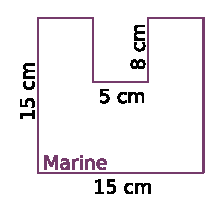
\includegraphics[width=.5\linewidth]{DiEa02}
    \end{center}
 
\item Ses amies Alison et Laura ont découpé des rectangles de largeur 5\,cm mais de longueurs différentes : celui d'Alison a une longueur de 6,3\,cm alors que celui de Laura a une longueur de 9,6\,cm. 
 
Calcule les périmètres des U d'Alison et de Laura. Quelle partie du calcul est la même pour tous les U ?

\item Après tous ces calculs, Kévin remarque que si $L$ désigne la longueur du rectangle en centimètres et $\mathcal{P}$ le périmètre du U en centimètres, alors  $\mathcal{P}= 60 + 2L$. Calcule $\mathcal{P}$ lorsque $L = 7,5$\,cm puis lorsque $L = 10$\,cm.
\item Priscilla dit : \og On peut encore simplifier : $60 + 2 = 62$ donc $\mathcal{P} = 62 L$. \fg. Utilise l'expression proposée par Priscilla pour calculer $\mathcal{P}$ lorsque $L = 10$\,cm. Qu'en déduis-tu ?
\end{colenumerate} 
\end{exercice}

\begin{exercice}[Distributivité à gogo]

\begin{colenumerate}{1} 
\item On veut développer l'expression $A = 2(5x + 2)(3x + 1)$. Pour cela, développe d'abord l'expression $2(5x + 2)$ puis termine le développement de $A$.
\item Développe le produit $(x + 2)(3x + 2)$ et déduis-en le développement de :
    \subitem $B = (x + 2)(3x + 2)(x + 4)$
\item En t'inspirant des questions précédentes, développe les expressions suivantes :
    \subitem $C = 4(5x -1)(3x + 3) $
    \subitem $D = (1 -x)(1 + x)(2x + 1)$
\end{colenumerate}
\end{exercice}




\begin{exercice}[Idée fausse]

\begin{colenumerate}{1} 
\item On considère les expressions $A = (2x + 3)^2$ et $B = (2x)^2 + 32$. Calcule ces expressions pour $x = 0$ et pour $x = 10$. Qu'en déduis-tu ?
\item Peut-on dire que pour tout nombre $a$ et tout nombre $b$ non nuls, les expressions $(a + b)^2$ et  $a^2 + b^2$ sont égales ? Justifie. Développe alors l'expression $(a + b)^2$.
\item On considère les deux expressions $C = (2x + 3) (2x -3)$ et $D = (2x)^2 -3^2$. Calcule ces expressions pour $x = 0$ puis pour $x = 10$. Qu'en déduis-tu ? Démontre-le.
\item Développe alors l'expression : $(a + b)(a -b)$.
\end{colenumerate} 
\end{exercice}



\begin{exercice}[Calcul mystère]

\begin{colenumerate}{1} 
\item \label{DisEA03} Calcule les expressions $2001 \times 1999 -2000^2$ et $47 \times 45 -46^2$. Que remarques-tu ?
\item Développe et réduis l'expression suivante :
\[(x + 1)(x -1) -x^2\]
\item Les résultats obtenus à la question \ref{DisEA03} étaient-ils prévisibles ? Justifie.
\item Écris d'autres expressions du même style et donne leurs résultats sans poser d'opération.
\end{colenumerate} 
\end{exercice}




\begin{exercice}[Petites démonstrations]

\begin{colenumerate}{1} 
\item Que dire de la somme de deux nombres pairs ? De deux nombres impairs ? Pourquoi ?
\item La somme de deux nombres consécutifs est‑elle paire ou impaire ? Justifie.
\item Que dire du produit de deux nombres pairs ? De deux nombres impairs ? De deux nombres consécutifs ? Pourquoi ?
\end{colenumerate} 
\end{exercice}



\serie{Problèmes}



\begin{exercice}[]
On considère les deux parallélépipèdes rectangles suivants :
    
    \begin{center}
    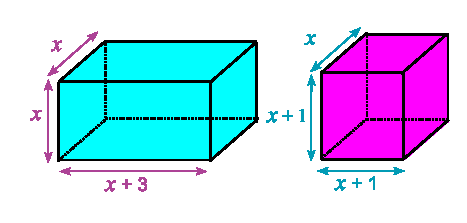
\includegraphics[width=.9\linewidth]{DiEa03}
    \end{center}

\begin{colenumerate}{1} 
\item \label{DisEA05} Calcule les deux volumes pour $x = 1$.

Que remarques-tu ?
\item Exprime, en fonction de $x$, les deux volumes. Que remarques-tu ? Comment expliquer alors le résultat de la question \ref{DisEA05} ?
\end{colenumerate} 
\end{exercice}




\begin{exercice}[]
On considère la figure suivante ($x$ désigne un nombre supérieur ou égal à 2) : 

    \begin{center}
    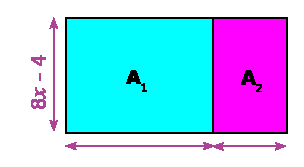
\includegraphics[width=.7\linewidth]{DiEa04}
    \end{center}

\begin{colenumerate}{1} 
\item Exprime en fonction de $x$ les aires $\mathcal{A}_1$ et $\mathcal{A}_2$.
\item Déduis-en une expression de l'aire totale $\mathcal{A}$ de la figure.
\item Calcule $\mathcal{A}_1$, $\mathcal{A}_2$ et $\mathcal{A}$ pour $x = 6$.
\end{colenumerate} 
\end{exercice}




\begin{exercice}[]
Isabelle achète $t$ kilogrammes d'oignons à 3,20\,€ le kilo et elle achète le double en masse de tomates à 2,30\,€ le kilo. Exprime, en fonction de $t$, le montant de ses achats en euros.
\end{exercice}



\begin{exercice}[]
Adeline achète 5 CD et 3 DVD. On notera $x$ le prix en euros d'un CD. Un DVD coûte 10 euros de plus qu'un CD.

\begin{colenumerate}{1} 
\item \label{DisEA06} Écris, en fonction de $x$, la dépense d'Adeline en euros. Développe et réduis l'expression trouvée.
\item En utilisant l'expression obtenue au \ref{DisEA06}, calcule, en euros, la dépense d'Adeline si un CD coûte 15\,€.
\end{colenumerate} 
 
\end{exercice}

\begin{exercice}[] 
La figure ci-dessous représente un carré de 6\,cm de côté. $M$ est un point de $[AD]$ et $N$ est un point de $[AB]$ tels que : 

$AM = AN = x$ ($x$ est un nombre strictement positif).

    \begin{center}
    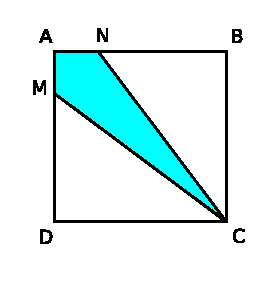
\includegraphics[width=.6\linewidth]{DiEa05}
    \end{center}

\begin{colenumerate}{1} 
\item Calculer, en fonction de $x$, les aires des triangles $MDC$ et $NBC$.
\item Calculer, en fonction de $x$, l'aire du quadrilatère $AMCN$.
\item Calculer ces trois aires pour $x = 2$\,cm. 
\end{colenumerate} 
\end{exercice}




\begin{exercice}[]
Une salle de concert peut contenir 600 places. Il y a $x$ places assises et les autres sont debout. Les places debout coûtent 15\,€ et les places assises 25\,€.

\begin{colenumerate}{1} 
\item Que représentent les expressions suivantes : $600 -x$ ; $25x$ et $15(600 -x)$ ?
\item Exprime, en fonction de $x$, la recette totale en euros si toutes les places sont prises.
\item Calcule cette recette si $x = 200$.
\end{colenumerate}
\end{exercice}
